%!TEX root = ./lec03_hardware.tex

%
% ---------------------------------------------------------------------------
%
\begin{frame}{DBMS Operational Requirements}


\vskip2em

The DBMS must meet these conflicting goals:

\vskip1em

\begin{columns}[onlytextwidth]
\begin{column}{0.475\textwidth}
\begin{BOX}{Preserving data}
To \textbf{preserve the data}, the DBMS must make sure that it is safely stored in persistent storage\footnotemark.
\end{BOX}
\end{column}
\begin{column}{0.475\textwidth}
\begin{BOX}{Using data}
Queries and updates are processed by the CPU!\\
 - the data needs to reach the registers
\end{BOX}
\end{column}
\end{columns}

\vskip1em

As a result: \alert{data is always on the move}.


\footnotetext{In fact, the privacy-conscious should note that it can be \emph{very hard} to erase data that has been properly written into persistent storage.}

\vskip2em
\end{frame}

%
% ---------------------------------------------------------------------------
%
\begin{frame}{How can the DBMS use persistent storage?}

\textbf{Option \#1}: via a File System:\footnote{\url{https://en.wikipedia.org/wiki/File_system}}\\
- there are many good file systems out there;\\
- however, they are optimized to handle a \emph{large number of small files}, logically organized into hierarchies (directories); databases typically have a \emph{small number of large tables}.

% \vskip1em

\textbf{Option \#2}: implementing \highlight{its own} I/O management:\\
- the Buffer Manager reads/writes directly from/to the device;\\
- requires integration with the Operating System kernel.\footnote{\url{https://en.wikipedia.org/wiki/Kernel_(operating_system)}}

\vskip0.5em

\underline{Most DBMSs have their own I/O stack}, and some require changing the Operating System to work.
\end{frame}


%
% ---------------------------------------------------------------------------
%
\begin{frame}

\begin{columns}[onlytextwidth]
\begin{column}{0.75\textwidth}
\vskip2em
\begin{BOX}{The Buffer Manager}

DBMS module responsible for moving data between storage and memory.

\vskip0.5em

It splits main memory into logical units called \emph{buffers}, which are often the same size of a memory page.
\end{BOX}
\vskip1em

Before data becomes visible to the CPU, it must be \emph{copied} in every level of the memory hierarchy!

\vskip1em
Because I/O is so slow, a badly designed Buffer Manager can make the DBMS unusable.
\end{column}
\begin{column}{0.2\textwidth}
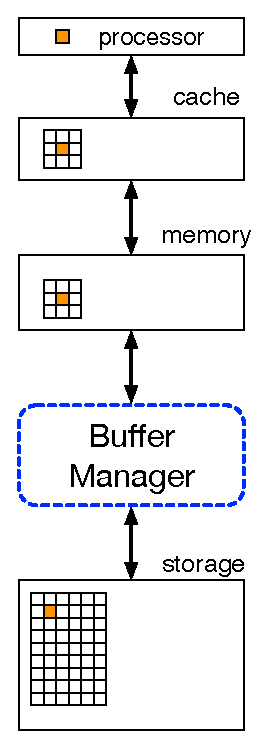
\includegraphics[width=\textwidth]{./figures/buffer_manager}
\end{column}
\end{columns}
\end{frame}

%
% ---------------------------------------------------------------------------
%
\begin{frame}
\begin{columns}[onlytextwidth]
\begin{column}{0.75\textwidth}
\vskip2em
\begin{BOX}{Updates}
When the processor changes an attribute of a tuple, the new value is modified in the cache and the memory first.
\end{BOX}

\vskip0.5em

\begin{BOX}{Insertions}
When a new tuple is inserted, it is stored in some buffer in memory first.\\
 -if there is no room in any buffer, a \emph{new one is created} in memory first.
\end{BOX}

\vfill

Any buffer containing data not yet on the storage layer is said to be \highlight{dirty}.
\end{column}
\begin{column}{0.2\textwidth}
\includegraphics[width=\textwidth]{./figures/buffer_manager_2}
\end{column}
\end{columns}
\end{frame}

%
% ---------------------------------------------------------------------------
%
\begin{frame}

\vskip2em

\begin{BOX}{Dirty data sits in volatile memory}
The Buffer Manager must \alert{\emph{flush} dirty buffers} to the storage layer for the changes to become persistent.
\end{BOX}

\vskip1em

Trade-off:
\begin{itemize}[-,topsep=-0.5em,noitemsep]
\item Because storage is so slow, it is a bad idea to flush dirty buffers \underline{immediately} after every insert/update.
\item The changes to the database do not become permanent \alert{until} they are written on persistent storage.
\end{itemize}



\end{frame}

%
% ---------------------------------------------------------------------------
%
\begin{frame}{Logging, Persistence and Recovery}

\vskip1em

\begin{columns}[onlytextwidth]
\begin{column}{0.6\textwidth}
The DBMS keeps a log of every modification (insertion, deletion, update) done to the database, \emph{on a separate} file (or even a separate storage device).

\vskip1em

Dirty buffers can safely remain in memory as soon as the changes are written to the log.

\vskip1em

If the computer crashes, all changes still in memory can be recovered from the log.
\end{column}
\begin{column}{0.4\textwidth}
\hspace*{2em}\includegraphics[width=\textwidth]{figures/buffer_manager_log_writer.eps}
\end{column}
\end{columns}
\end{frame}



%
% ---------------------------------------------------------------------------
%
% ---------------------- get the tuplex from the example tables

\newsavebox\MovieI
\savebox{\MovieI}{
	\clipbox{0 45.125 0 22.125}{\usebox\MovieTable}
}
\newsavebox\MovieII
\savebox{\MovieII}{
	\clipbox{0 33.75 0 33.45}{\usebox\MovieTable}
}
\newsavebox\MovieIII
\savebox{\MovieIII}{
	\clipbox{0 22.65 0 44.75}{\usebox\MovieTable}
}
\newsavebox\MovieIV
\savebox{\MovieIV}{
	\clipbox{0 11.3 0 56}{\usebox\MovieTable}
}
\newsavebox\MovieV
\savebox{\MovieV}{
	\clipbox{0 0 0 67.25}{\usebox\MovieTable}
}

\newsavebox\MovieVI
\savebox{\MovieVI}{
	\clipbox{0 0 0 33.5}{\usebox\MovieTableTWO}
}

\def\movieTupleGHOSTBUSTERSone{\scalebox{0.75}{\usebox{\MovieI}}}
\def\movieTupleBIG{\scalebox{0.75}{\usebox{\MovieII}}}
\def\movieTupleLOSTinTRANSLATION{\scalebox{0.75}{\usebox{\MovieIII}}}
\def\movieTupleWADJDA{\scalebox{0.75}{\usebox{\MovieIV}}}
\def\movieTupleGHOSTBUSTERStwo{\scalebox{0.75}{\usebox{\MovieV}}}
\def\movieTupleGROUNDHOGday{\scalebox{0.75}{\usebox{\MovieVI}}}

\def\idxKeyTitleBIG{\scalebox{0.75}{\clipbox{5 0 140 0}{\usebox\MovieII}}}
\def\idxKeyTitleGHOSTBUSTERSone{\scalebox{0.75}{\clipbox{5 0 140 0}{\usebox\MovieI}}}
\def\idxKeyTitleGHOSTBUSTERStwo{\scalebox{0.75}{\clipbox{5 0 140 0}{\usebox\MovieV}}}
\def\idxKeyTitleLOSTinTRANSLATION{\scalebox{0.75}{\clipbox{5 0 140 0}{\usebox\MovieIII}}}
\def\idxKeyTitleWADJDA{\scalebox{0.75}{\clipbox{5 0 140 0}{\usebox\MovieIV}}}

\def\idxKeyTitleYearBIG{\scalebox{0.75}{\clipbox{8 0 111 0}{\usebox\MovieII}}}
\def\idxKeyTitleYearGHOSTBUSTERSone{\scalebox{0.75}{\clipbox{8 0 111 0}{\usebox\MovieI}}}
\def\idxKeyTitleYearGHOSTBUSTERStwo{\scalebox{0.75}{\clipbox{8 0 111 0}{\usebox\MovieV}}}
\def\idxKeyTitleYearLOSTinTRANSLATION{\scalebox{0.75}{\clipbox{8 0 111 0}{\usebox\MovieIII}}}
\def\idxKeyTitleYearWADJDA{\scalebox{0.75}{\clipbox{8 0 111 0}{\usebox\MovieIV}}}


% -------------------------- macros for drawing tuples in the data file

\tikzset{
	tuple/.style={
		anchor=north west,
		inner sep=0pt,outer sep=0pt,shift={(0pt,-2pt)}
	}
}

\tikzset{ % same as above, except for the anchor part
	tupleBelow/.style={
		inner sep=0pt,outer sep=0pt,shift={(0pt,-2pt)}
	}
}


% #1     --> id of tuple (i.e., the node with the value)
% #2, #3 --> coordinages of top-left corner of node with tuple value
% #4     --> value in the attribute of the tuple
\def\tuple#1#2#3#4{
  \node ({#1}) at ({#2},{#3}) [tuple] {{#4}} ;
}

% #1     --> id of tuple (i.e., the node with the value)
% #2, #3 --> coordinages of top-left corner of node with tuple value
% #4     --> value in the attribute of the tuple
\def\tupleBelow#1#2#3{
  \node ({#1}) [below = -2pt of {#2}] [tupleBelow] {{#3}} ;
}


% --------------------------- macros for drawing blocks of the data file

\tikzset{
	MovieDataBlock/.style={
		draw,rectangle,minimum width=5.5125cm, minimum height=0.69cm,anchor=north west,inner sep=1pt,outer sep=1pt
	}
}

\tikzset{
	MovieDataBlockPointerBox/.style={
		fill=snow,draw,rectangle,minimum width=1em,minimum height=1em,
		anchor=north west,
		inner sep=1pt,outer sep=1pt,
		shift={(5.5125cm,-0.34cm)}
	}
}


% #1    --> block id
% #2,#3 --> coordinates of top-left corner
% #4    --> id of the first tuple
% #5    --> value of the first tuple
\def\movieDataBlock#1#2#3#4#5{
	\node ({#1}) at ({#2},{#3}) [MovieDataBlock] {};
	\node at ({#2},{#3}) [MovieDataBlockPointerBox] {};
	
	\tuple{#4}{#2}{#3}{#5};
}

% #1     --> block id
% #2     --> id of block ``above'' this one
% #3, #4 --> coordinates of this block
% #5     --> id of the first tuple inside the block
% #6     --> value of the first tuple
\def\movieDataBlockBelow#1#2#3#4#5#6{
	\node ({#1}) at ({#3},{#4}) [MovieDataBlock] {};
	\node at ({#3},{#4}) [MovieDataBlockPointerBox] {};
	\draw [*->] ([xshift=4pt,yshift=8pt]{#2}.south east) to[out=270,in=90] ([xshift=-10pt]#1.north east);

	\tuple{#5}{#3}{#4}{#6};
}


% --------------------------- macros for drawing the keypointer pairs in the index

\tikzset{
	indexKeyBox/.style={
		anchor=north west,
		inner sep=0pt,outer sep=0pt,shift={(2pt,-2pt)}
	}
}

\tikzset{ %same as above, except for the anchor point
	indexKeyBelowBox/.style={ 
		inner sep=0pt,outer sep=0pt
	}
}

\tikzset{
	indexPointerBox/.style={
		fill=snow,draw,rectangle,minimum width=0.75cm,minimum height=0.3cm,
		inner sep=1pt,outer sep=1pt
	}
}

% draws two rectangles, one with an attribute value, the other with the pointer
%
% #1     --> id of key-pointer (i.e., the node with the value)
% #2, #3 --> coordinages of top-left corner of node with tuple value
% #4     --> value in the attribute of the tuple
\def\movieIndexKeyPointer#1#2#3#4{
  \node ({#1}) at ({#2},{#3}) [indexKeyBox] {#4} ;
  \node [right = -0.5pt of {#1}] [indexPointerBox] {};
}

% #1     --> id of key-pointer (i.e., the node with the value)
% #2     --> id of key-pointer immediately above
% #4     --> value in the attribute of the tuple
\def\movieIndexKeyPointerBelow#1#2#3{
  \node ({#1}) [below = -0.5pt of {#2}] [indexKeyBelowBox] {\tiny{#3}} ;
  \node [right = -0.5pt of {#1}] [indexPointerBox] {};
}


% --------------------------- macros for drawing blocks of the index file

\tikzset{
	MovieIndexBlock/.style={
		draw,rectangle,anchor=north west,inner sep=1pt,outer sep=1pt
	}
}

\tikzset{
	MovieIndexBlockPointerBox/.style={
		fill=snow,draw,rectangle,minimum height=1em,minimum width=1em,
		anchor=north west,
		inner sep=0pt,outer sep=0pt
	}
}

% #1    --> block id
% #2,#3 --> coordinates of top-left corner
% #4    --> WIDTH of block box
% #5    --> HEIGHT of the block box
% #6    --> id of the key-pointer pair
% #7    --> value of the first key-pointer pair
\def\movieIndexBlock#1#2#3#4#5#6#7{
	\node ({#1}) at ({#2},{#3}) [minimum width={#4},minimum height={#5},MovieIndexBlock] {};
	\node [below left= 0pt and 0pt of {#1}] [shift={(-0.9em,1.1em)},MovieIndexBlockPointerBox] {};

	\movieIndexKeyPointer{#6}{#2}{#3}{#7};
}

% #1    --> block id
% #2    --> id of block above
% #3,#4 --> coordinates of top-left corner
% #5    --> WIDTH of block box
% #6    --> HEIGHT of the block box
% #7    --> id of the key-pointer pair
% #8    --> value of the first key-pointer pair
\def\movieIndexBlockBelow#1#2#3#4#5#6#7#8{
	\node ({#1}) at ({#3},{#4}) [minimum width={#5},minimum height={#6},MovieIndexBlock] {};
	\node [below left= 0pt and 0pt of {#1}] [shift={(-0.9em,1.1em)},MovieIndexBlockPointerBox] {};
	\draw [*->] ([xshift=-0.4em,yshift=0.8em]{#2}.south west) to[out=270,in=90] ([xshift=10pt]{#1}.north west);

	\movieIndexKeyPointer{#7}{#3}{#4}{#8};
}


% ----------------------------- draw line between pointer into tuple

% #1 --> key-pointer id
% #2 --> tuple id
\def\KPtoTuple#1#2{
	\draw [*->] ([xshift=0.35cm,yshift=0em]{#1}.east) to[out=0,in=180] (#2.west);
}

% ======================== actual examples

\newsavebox\TitleIndexOnMovie
\savebox{\TitleIndexOnMovie}{
\begin{tikzpicture}
\movieDataBlock{Mdb1}{0}{0}{t1}{\movieTupleGHOSTBUSTERSone};
\tupleBelow{t2}{t1}{\movieTupleBIG};
\movieDataBlockBelow{Mdb2}{Mdb1}{0}{-1.25}{t3}{\movieTupleLOSTinTRANSLATION};
\tupleBelow{t4}{t3}{\movieTupleWADJDA};
\movieDataBlockBelow{Mdb3}{Mdb2}{0}{-2.5}{t5}{\movieTupleGHOSTBUSTERStwo};

\movieIndexBlock{MIb1}{-4.5}{0}{7.6em}{3.6em}{kp1}{\idxKeyTitleBIG};
\movieIndexKeyPointerBelow{kp2}{kp1}{\idxKeyTitleGHOSTBUSTERSone};
\movieIndexKeyPointerBelow{kp3}{kp2}{\idxKeyTitleGHOSTBUSTERStwo};
\movieIndexKeyPointerBelow{kp4}{kp3}{\idxKeyTitleLOSTinTRANSLATION};
\movieIndexBlockBelow{MIb2}{MIb1}{-4.5}{-2.25}{7.6em}{3.6em}{kp5}{\idxKeyTitleWADJDA};

\KPtoTuple{kp2}{t1};
\KPtoTuple{kp1}{t2};
\KPtoTuple{kp4}{t3};
\KPtoTuple{kp5}{t4};
\KPtoTuple{kp3}{t5};
\end{tikzpicture}}


\newsavebox\TitleYearIndexOnMovie
\savebox{\TitleYearIndexOnMovie}{
\begin{tikzpicture}
\movieDataBlock{Mdb1}{0}{0}{t1}{\movieTupleGHOSTBUSTERSone};
\tupleBelow{t2}{t1}{\movieTupleBIG};
\movieDataBlockBelow{Mdb2}{Mdb1}{0}{-1.25}{t3}{\movieTupleLOSTinTRANSLATION};
\tupleBelow{t4}{t3}{\movieTupleWADJDA};
\movieDataBlockBelow{Mdb3}{Mdb2}{0}{-2.5}{t5}{\movieTupleGHOSTBUSTERStwo};

\movieIndexBlock{MIb1}{-4.5}{0}{9.6em}{2.8em}{kp1}{\idxKeyTitleYearBIG};
\movieIndexKeyPointerBelow{kp2}{kp1}{\idxKeyTitleYearGHOSTBUSTERSone};
\movieIndexKeyPointerBelow{kp3}{kp2}{\idxKeyTitleYearGHOSTBUSTERStwo};

\movieIndexBlockBelow{MIb2}{MIb1}{-4.5}{-2.25}{9.6em}{2.8em}{kp4}{\idxKeyTitleYearLOSTinTRANSLATION};
\movieIndexKeyPointerBelow{kp5}{kp4}{\idxKeyTitleYearWADJDA};

\KPtoTuple{kp2}{t1};
\KPtoTuple{kp1}{t2};
\KPtoTuple{kp4}{t3};
\KPtoTuple{kp5}{t4};
\KPtoTuple{kp3}{t5};
\end{tikzpicture}}


\newsavebox\SequentialFileMovieTitleYear
\savebox{\SequentialFileMovieTitleYear}{
\begin{tikzpicture}
\movieDataBlock{Mdb1}{0}{0}{t1}{\movieTupleBIG};
\tupleBelow{t2}{t1}{\movieTupleGHOSTBUSTERSone};
\movieDataBlockBelow{Mdb2}{Mdb1}{0}{-1.25}{t3}{\movieTupleGHOSTBUSTERStwo};
\tupleBelow{t4}{t3}{\movieTupleLOSTinTRANSLATION};
\movieDataBlockBelow{Mdb3}{Mdb2}{0}{-2.5}{t5}{\movieTupleWADJDA};
\end{tikzpicture}}

\newsavebox\SequentialFileMovieTitlYearUpdated
\savebox{\SequentialFileMovieTitlYearUpdated}{
\begin{tikzpicture}
\movieDataBlock{Mdb1}{0}{0}{t1}{\movieTupleBIG};
\tupleBelow{t2}{t1}{\movieTupleGHOSTBUSTERSone};
\movieDataBlockBelow{Mdb2}{Mdb1}{0}{-1.25}{t3}{\movieTupleGHOSTBUSTERStwo};
\tupleBelow{t4}{t3}{\movieTupleGROUNDHOGday};
\movieDataBlockBelow{Mdb3}{Mdb2}{0}{-2.5}{t5}{\movieTupleLOSTinTRANSLATION};
\tupleBelow{t6}{t5}{\movieTupleWADJDA};
\end{tikzpicture}}

\newsavebox\SequentialFileMovieTitlYearUpdatedTWO
\savebox{\SequentialFileMovieTitlYearUpdatedTWO}{
\begin{tikzpicture}
\movieDataBlock{Mdb1}{0}{0}{t1}{\movieTupleBIG};
\tupleBelow{t2}{t1}{\movieTupleGHOSTBUSTERSone};
\movieDataBlockBelow{Mdb2}{Mdb1}{0}{-1.25}{t3}{\movieTupleGHOSTBUSTERStwo};
\movieDataBlockBelow{Mdb3}{Mdb2}{0}{-2.5}{t4}{\movieTupleGROUNDHOGday};
\tupleBelow{t5}{t4}{\movieTupleLOSTinTRANSLATION};
\movieDataBlockBelow{Mdb4}{Mdb3}{0}{-3.75}{t6}{\movieTupleWADJDA};
\end{tikzpicture}}



\begin{frame}{Database ``Files''?}

Tables are collections of records stored on ``files'' (chains of fixed-sized blocks). Indexes help the DBMS find tuples through pointers.


\begin{tikzpicture}
\node [anchor=north west] at (-0.15,0) {\scalebox{0.85}{\usebox\TitleYearIndexOnMovie}};
\node [color=accent] at (1,0.5) {Index File};
\node [color=accent] at (5,0.5) {Table File};
\end{tikzpicture}

A ``database pointer'' identifies the storage device \emph{and} a block address which can be translated into a device-specific address (recall slide~\ref{block_oriented_storage}).

\end{frame}


%
% ---------------------------------------------------------------------------
%
\begin{frame}{Main Memory Databases}

Some DBMSs (including SQLite) are optimized for main memory and use only virtual memory as its address space.

This is rarely a problem, as Virtual Memory can grow to Petabytes (recall Slide~\ref{virtual_memory_size}) with modern computers.

In any case, relying on virtual memory as the database address space simplifies the DBMS architecture a lot. For example ``database'' pointers can be simplified to virtual memory addresses.

Main-memory DBMSs are also optimized for single-user applications (like mobile applications and video games).

\end{frame}


%
% ---------------------------------------------------------------------------
%
\begin{frame}{What about bigger databases?}

A very small number of applications (and organizations) deal with more than a Petabyte. In such cases, we need clusters of high-performance computers and (often) a custom DBMS.

\begin{center}
\begin{tikzpicture}
\node at (0,0) [anchor=south east] {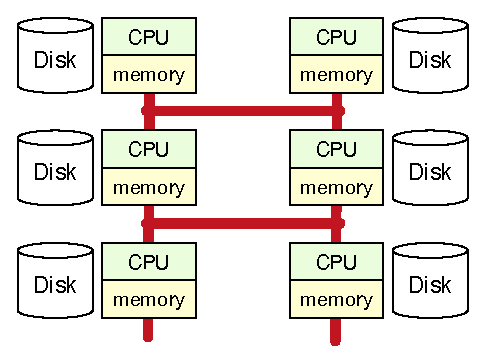
\includegraphics[width=0.4\textwidth]{figures/small_cluster.eps}};
\end{tikzpicture}
\end{center}

In such cases, to identify a tuple we need to know:\\
 - the specific block of a specific storage device holding the tuple\\
 - the IP address of the server with that device (if using a cluster)


\end{frame}


%
% ---------------------------------------------------------------------------
%
\begin{frame}

The standard DBMS implementations use \alert{\textbf{symbolic}} pointers, even for single CPU DBMSs.

Symbolic addresses are typically \underline{much larger} than a memory address. 
Also, symbolic addresses \alert{\textbf{must be resolved}} into virtual memory addresses!

\vskip1.5em

\begin{BOX}{Resolving pointers as blocks are loaded...}
When the Buffer Manager loads a symbolic pointer to memory, it must translate that symbolic address to an actual \emph{virtual memory} address where the target of the link is actually loaded.
\end{BOX}
\end{frame}
